\subsection{Information Visualization} \label{sec:vis_dr}
We define `information visualization' as the act of displaying artifacts generated by AIA models or processes for the task at hand in such a way as to communicate to one of the trust dimensions of a human user. Specifically we consider the `competence' and `predictability' of the AIA, as well as the `situational normality' of the task at hand. This can overlap but is not necessarily the same as generating self-assessments, which are introspective and \emph{process based} assurances (i.e. which are descriptive and reflective of the AIA's capabilities); rather, information visualization tends to more broadly include or revolve around \emph{outcome based} assurances (i.e. which focus on results or expected results of applying the AIA's capabilities).  

\subsubsection{Common Approaches:}
\citet{Liu2017-xw} review several of the current methods that exist for visualizing machine learning models. They identified three main purposes for which visualizations are useful in this context: 1) understanding (why models behave the way they do on certain problems), 2) diagnosis (failures, or unexpected behavior on certain tasks), and 3) refinement (ability to improve performance on tasks). 
We consider two common methods that assist in these processes: dimensionality reduction and visualization of uncertainty.

\paragraph{Dimensionality Reduction:}
Dimensionality reduction (DR) is one of the key methods used in creating visualizations. \citet{Sacha2017-hf} identify seven different methods by which users interact with DR techniques. They use this to make the human-in-the-loop process model for interactive DR that is shown in Figure~\ref{fig:sacha_fig}. This interactive nature of their model helps users to better understand the information that they are viewing.

\begin{figure}[htpb]
    \centering
    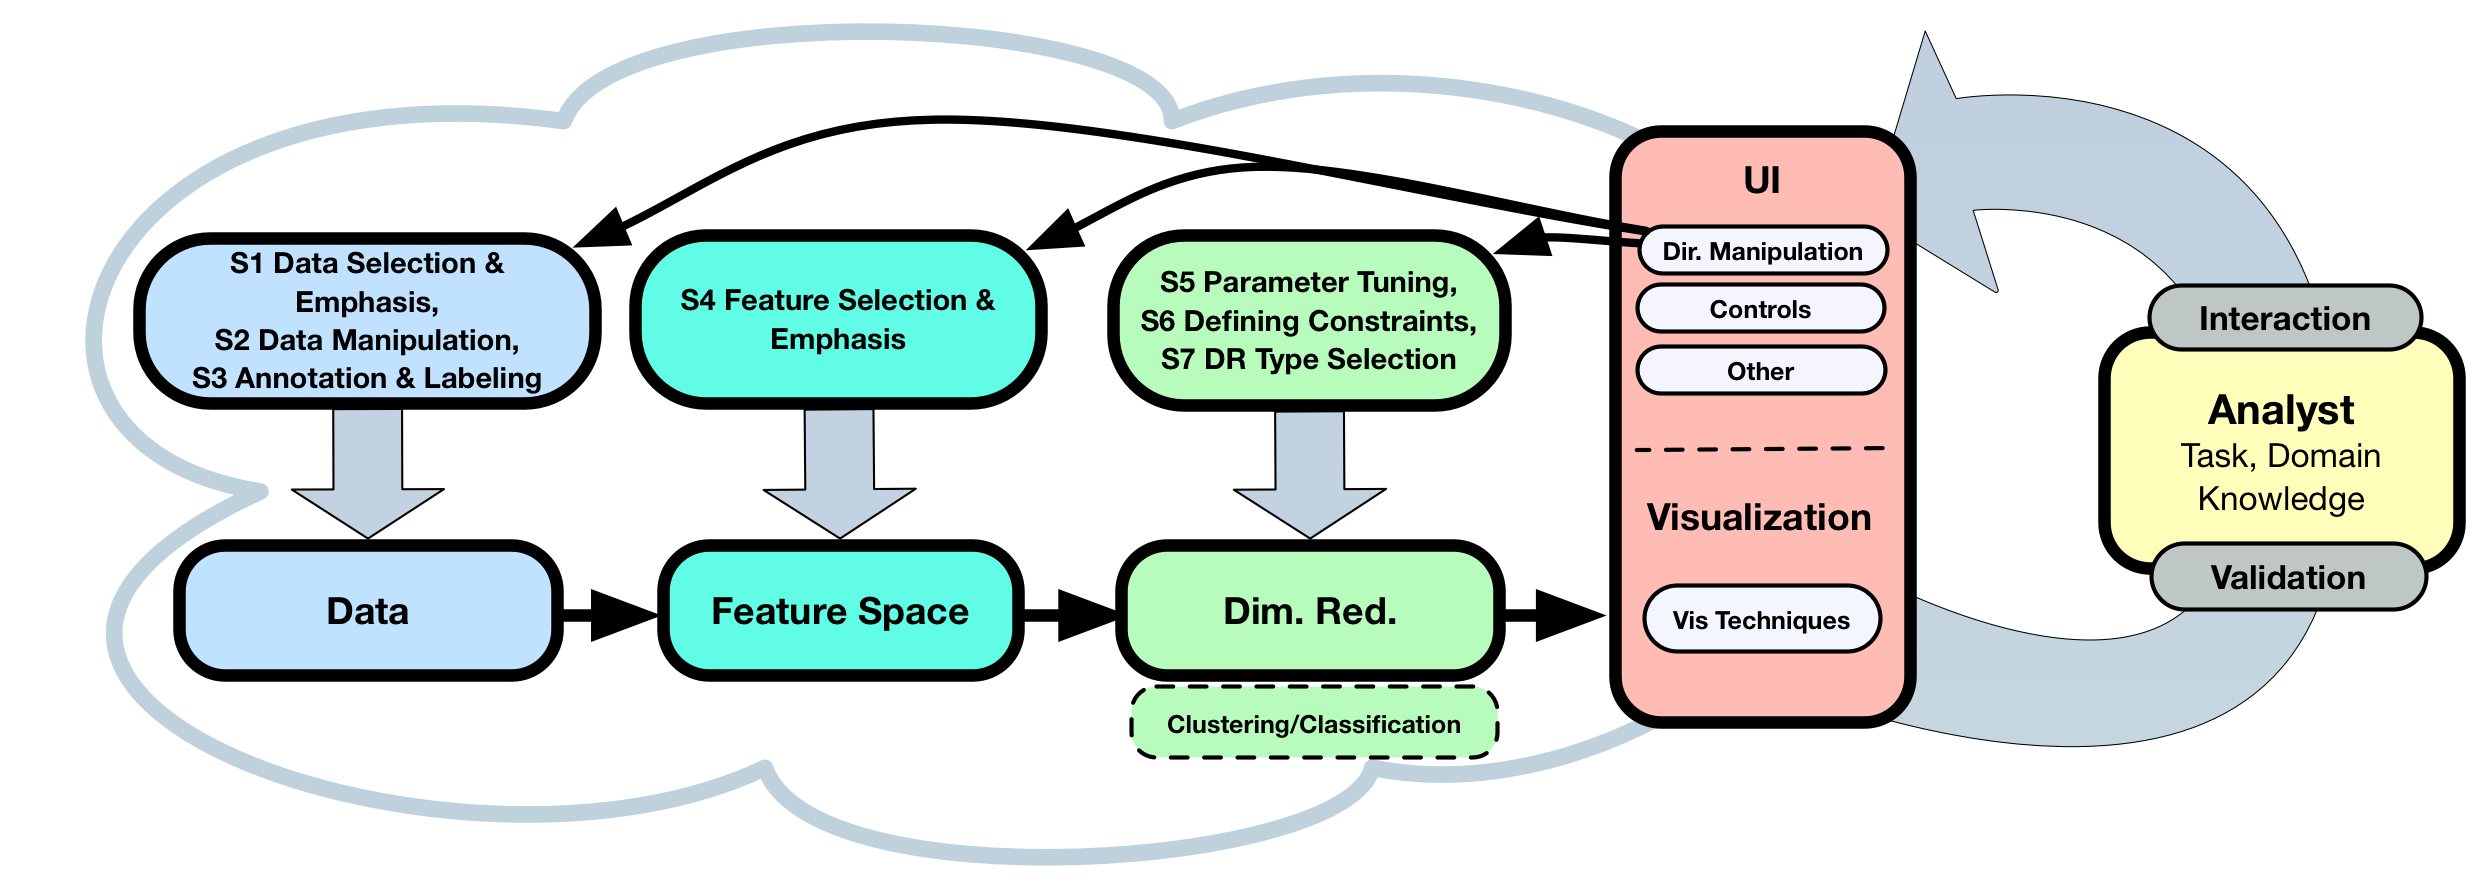
\includegraphics[width=0.8\linewidth]{Figures/dimred_framework.png}
    \caption{Human-in-the-loop process model proposed by \cite{Sacha2017-hf}. Included by permission.}
    \label{fig:sacha_fig}
\end{figure}

\citet{Venna2007-yj} discusses DR for ML and reviews many linear and non-linear projection methods. \citet{Vellido2012-nm} also discusses the importance of DR for making ML models interpretable. As one example, \citet{Chipman2005-om} applied this idea by constraining principle component analysis (PCA) in an attempt to make the resulting linear combinations of variables more interpretable (more homogeneous, or more sparse).

At times a simple visualization is the most efficient way to communicate the results of decision making or planning. For example: \citet{Chadalavada2015-wx} enable a robot to project its path onto the ground so users can see.

\paragraph{Treatment of Uncertainty:}
In the previous section we have already visited the importance of an AIA being able to quantify its uncertainty. Visualization researchers are concerned with how to \emph{convey} that uncertainty to human users (and quantify uncertainty inherent in making visualizations). \citet{Sacha2016-tu} discuss how the propagation of uncertainty through visual analytics systems can affect the trust of human users (see also \cite{Correa2009-hi}).
One excellent example of this is the work by \citet{Wu2012-qi}, who create a tool to visualize the flow and propagation of uncertainty in the visualization process. In this way users can understand where uncertainty enters the data visualization process.

The relationship between systemic uncertainties and their effects on system performance can be very complex. \citet{Hutchins2015-if} address this by using expert knowledge, and a `trust annunciator panel' (TAP) that has several `uncertainty level indicators' in order to display how uncertainties in sensors will effect the output quality, and the mission impact; and the same for the planning algorithm (see Figure~\ref{fig:hutchins_fig}).

\begin{figure}[htpb]
    \centering
    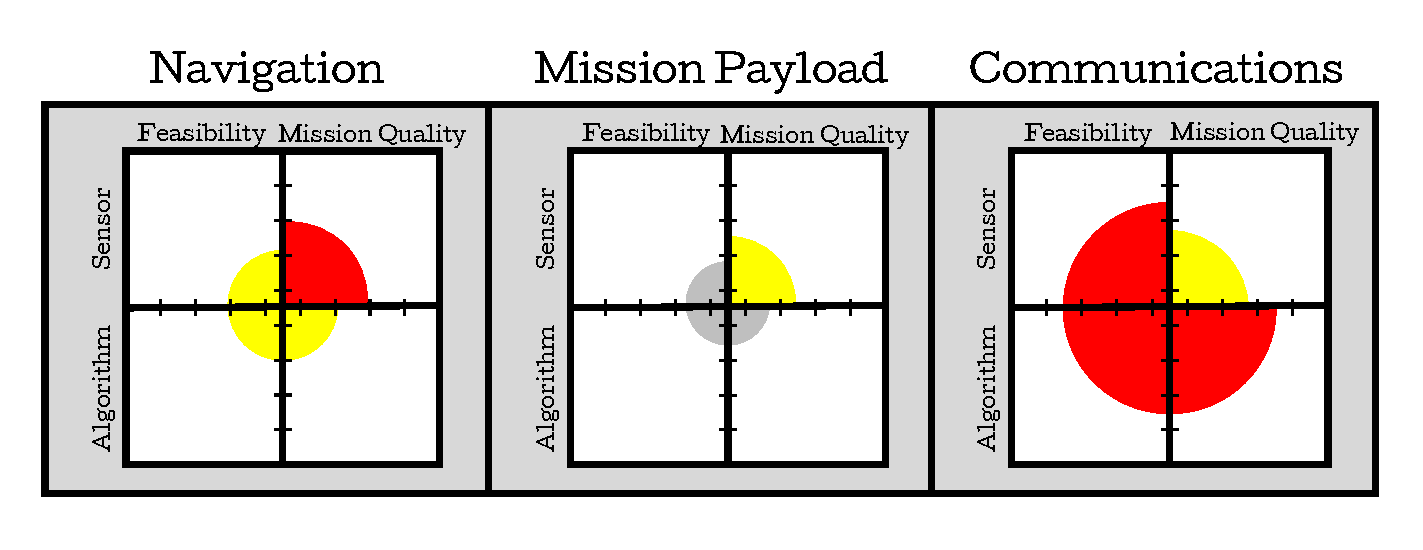
\includegraphics[width=0.7\linewidth]{Figures/Hutchins_fig.pdf}
    \caption{Proposed `trust annunciator panel' \cite{Hutchins2015-if}. Included by permission.}
    \label{fig:hutchins_fig}
\end{figure}

\subsubsection{Grounding Example:}
In the case of the `VIP Escort' problem (described in Section~\ref{sec:mot_example}), information visualization might be used as an assurance in the following way, starting with the assumptions that:

\begin{itemize}
    \item The UGV has just begun an attempt to escape the road-network
    \item The user has access to an interface like that proposed in \cite{Hutchins2015-if}
\end{itemize}

During the attempt the user is able to see how the sensor uncertainty might possibly effect the outcome of the mission. In this case, the user is assured that the sensors will have little negative impact on the outcome of the mission given the current weather conditions.

\paragraph{\textbf{Discussion of Example:}} Here we see how a visualization is able to assist the user in correlating the effects between sensor uncertainty and mission outcome. This is not a simple relationship for operators (especially untrained) to learn on their own; even if they were able to learn the time required to do so can be very detrimental.
